\documentclass[12pt,a4paper]{article}
\usepackage[utf8]{inputenc}
\usepackage[english]{babel}
\usepackage{amsmath}
\usepackage{amsfonts}
\usepackage{amssymb}
\usepackage{latexsym}
\usepackage{makeidx}
\usepackage{graphicx}
\usepackage{graphics}
\usepackage{lmodern}
\usepackage{hyperref}
\usepackage{subcaption}
\usepackage{pgfplots}
\usepackage{dsfont}
\usepackage{multicol}
\usepackage{xcolor}
\usepackage{booktabs}
\usepackage{float}
\usepackage{subcaption}
\pgfplotsset{width=10cm,compat=1.9}
\usepgfplotslibrary{external}
\usepackage{fancybox}
\usepackage{subcaption}


\setlength{\parindent}{0px}
\usepackage[left=2cm,right=2cm,top=4cm,bottom=2cm]{geometry}

\author{Daniel Vázquez Lago}
\title{Medida de la constante dieléctrica}

\newcommand{\parentesis}[1]{\left( #1  \right)}
\newcommand{\parciales}[2]{\frac{\partial #1}{\partial #2}}
\newcommand{\pparciales}[2]{\parentesis{\parciales{#1}{#2}}}
\newcommand{\ccorchetes}[1]{\left[ #1  \right]}
\newcommand{\D}{\mathrm{d}}
\newcommand{\sech}{\mathrm{sech} \ }
\newcommand{\csch}{\mathrm{csch} \ }

\begin{document}

\maketitle

\newpage

\tableofcontents

\newpage

\section{Objetivos}

El objetivo de está práctica será el cálculo de permitividad del vacío y la permitividad relativa de una placa de plástico. 

\section{Introducción}

Sabemos que la capacidad de un condensador de caras paralelas (con aire entre las placas) viene dado por:

\begin{equation}
C_0 = \dfrac{\varepsilon_0 S}{d} \label{Ec:1}
\end{equation}

siendo $S$ la superficie de las caras, $d$ la distancia entre las placas y $\varepsilon_0$ la permitividad del vacío. En el caso de que la entre las placas no haya aire, si no otro material con una permeatividad relativa $\varepsilon_r$ tendremos que la capacidad de nuestro condensador vendrá dado por:

\begin{equation}
C = \dfrac{\varepsilon_r \varepsilon_0 S}{d} \label{Ec:2}
\end{equation}

También sabemos que la capacidad de un condensador $C$ está definida según la  siguiente ecuación:

\begin{equation}
C = \dfrac{Q}{V} \label{Ec:3}
\end{equation}

donde $Q$ es la carga de la superficie del condensador y es la $V$ de potencial entre las superficies. Entonces si conocemos la capacidad del condensador en presencia del aire y en presencia del dieléctrico podremos obtener muy fácilmente la permeatividad relativa del medio, ya que será el cociente entre estas:

\begin{equation}
\varepsilon_r = \dfrac{C}{C_0} \label{Ec:cociente}
\end{equation}

Sin embargo el calculo de las cargas para calcular las capacidades conllevan un problema: para potenciales de $\Delta V$ pequeños como $10 V$ la carga almacenada $Q$ es muy pequeña. Sin embargo si le damos más potencia el aire comenzará a comportarse como un conductor, lo que puede crear descargas y otros problemas. Por eso buscaremos una forma de darle un potencial apreciable sin que ocurra esto. Para eso tendremos que montar un sistema que nos permita calcular la carga y la diferencia de potencial sin que haya ningún tipo de descarga o caída de potencial. 


\section{Material}

Además de mencionar el material usado, mencionaremos aquí cual es la incertidumbre de medida dada para cada objeto por el fabricante.

\begin{itemize}

\item \textbf{Condensador de placas paralelas:} a su capacidad la denotaremos como $C_P$, a la carga que adquieren sus placas por $Q_0$ y la diferencia de potencial entre las placas será $V_0$. Las caras serán circunferencias de radio $r=130 mm$, y el espacio entre las placas será regulable (incluye una escala que nos permite calcular dicha distancia).

\item \textbf{Condensador de medida:} a su capacidad la denotaremos como $C_M$ y tendrá el valor de $C_M = 220 nF$. A la carga de las superficie y potencial entre ellas las llamaremos $Q_M$ y $V_M$. Además tendremos que $C_M \gg C_P$. El condensador de Phywe tiene una tolerancia del $20\%$, que podemos consultar en su página web.

\item \textbf{Fuente de alta tensión:} suministrará una corriente continua con un potencial de 1 a 5 $kV$. La tensión que le demos será conocida en todo momento gracias a una pantalla. Según Phywe el generador de CC tendrá una variación máxima del $6\%$, que podemos encontrar en la página web.

\item \textbf{Resistencia:} se conecta en serie con la fuente por razones de seguridad (la resistencia tendrá $10 M \Omega$).

\item \textbf{Amplificador de medida:} el amplificador de medida nos permite medir el potencial entre las placas del condensador $C_M$ sin descargar el condensador. Su alta impedancia evita que se descargue, y como es de ganancia unidad, la señal que llega al polímetro será la misma que la que entra por el amplificador. Constará de un botón de descarga que pone a cero el potencial de entrada, es decir, elimina toda al carga $Q_M$.

\item \textbf{Polímetro:} con el se medirá la diferencia de potencial entre las caras del condensador $C_M$. El multímetro ``Electro Tools Multímetro Digital Compacto ET0830'' tendrá una incertidumbre, para las medidas de voltaje CC del $0.5\%+2$, que pudimos consultar en su hoja del fabricante.

\item Evidentemente tendremos varios cables de conexión y otros de alta tensión que nos permita conectar todo el circuito eléctrico, con las mínimas pérdidas.

\end{itemize}


\section{Montaje experimental}

El montaje experimental llevado acabo en está práctica tendrá como objetivo el cálculo de la carga $Q_P$ del condensador. Para esto alternaremos a lo largo del experimento entre dos configuraciones. Según a que circuito conectemos el condensador $C_P$ estaremos en la configuración 1 o 2:

\begin{itemize}
\item \textbf{Configuración 1.} En está configuración conectaremos el condensador a la fuente de alta tensión con una tensión $V_0$ conocida y a tierra. La carga que adquirirá nuestro medio será de $Q_0 = C_P V_0$. Véase figura \ref{Fig:cofiguracion1}.

\item \textbf{Configuración 2.} En está configuración conectamos el condensador al condensador de medida $C_M$ descargado (que esté descargado es vital). Dado que $C_M \gg C_P$, prácticamente toda la carga $Q_0$ almacenada en $C_P$ pasará a $C_M$. El cambio de una configuración a otra se realizará rápidamente para evitar descargas de $Q_0$. Además tendremos el amplificador de medida y un polímetro conectados en paralelo a nuestro que nos mida la diferencia de potencial del condensador $V_M$. Véase figura \ref{Fig:configuracion2}.
\end{itemize}

Dado que $Q_P \approx Q_M$, y que $Q_M = C_M V_M$ podremos calcular $Q_P$ midiendo la diferencia de potencial entre las superficies del condensador de medida.

\newpage


\begin{figure} \centering
\begin{subfigure}[b]{0.35\linewidth}
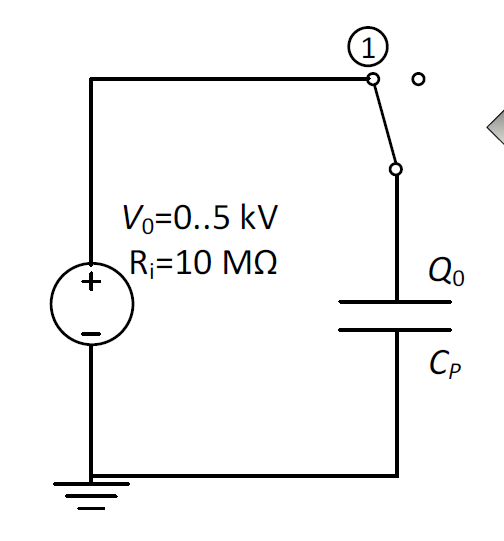
\includegraphics[width=\linewidth]{configuracion1.png}
\caption{Configuración 1}
\label{Fig:cofiguracion1}
\end{subfigure}
\begin{subfigure}[b]{0.558\linewidth}
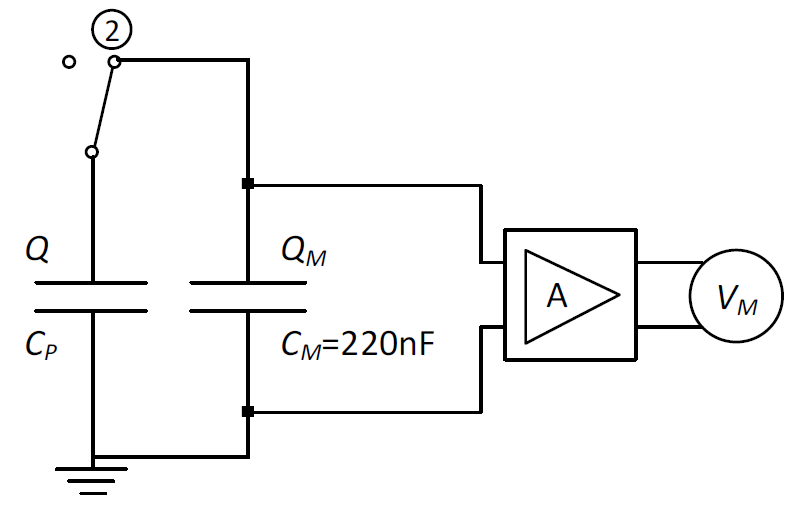
\includegraphics[width=\linewidth]{configuracion2.png}
\caption{Configuracion 2}
\label{Fig:configuracion2}
\end{subfigure}
\caption{circuitos de ambas configuraciones. Consultar bibliografía (sec. \ref{Sec:7}) para ver autoría.}
\end{figure}


\section{Procedimiento experimental}

En está sección explicaremos paso por paso que vamos haciendo a lo largo de la práctica, ya que entender como vamos a tomar los datos y con que lo vamos a hacer es fundamental para conocer las fuentes de incertidumbres y como se propagan. \\

Hay que resaltar que cada toma de datos se hará de manera análoga en todo el experimento: de existir un error sistemático se hará en cada una de las partes. Lo único que variará de una toma de datos a otra será la distancia entre las placas o el voltaje $V_0$ que le demos a nuestro generador. \\

La toma de datos se hará asi:

\begin{enumerate}
\item Se descarga los condensadores. Esto se hace teniendo la configuración 2 y usando en amplificador de medida. En el caso de no tenerlos descargados o no descargarlos quedará una carga remanente en $C_M$, que luego cuando volvamos a conectar ambos condensadores se sumará a la carga $Q_0$ y $Q_0 \approx Q_M$.

\item Una vez tenemos los condensadores descargados, dispondremos la configuración 1. Ahora una vez fijada la distancia que queramos, encendemos la fuente y la escogemos el potencial $V_0$.

\item Una vez se haya cargado el condensador (si el medio entre las caras es aire esto lleva unos pocos segundos, si es el plástico puede tardar un par de minutos), debemos pasar a la configuración dos. Como ya mencionamos, el cambio de configuración se debe hacer rápido, y de manera cuidadosa (recordemos que llegado un punto el aire comienza a tener un comportamiento similar a un conductor). 

\item Finalmente mediremos la diferencia de potencial entre las placas del condensador $C_M$ mediante el polímetro.

\end{enumerate}

Entonces haremos las siguientes partes:

\begin{itemize}
\item \textbf{Parte 1:} en la primera parte dejaremos fijo $V_0=1kV$, cambiando la distancia, tomando desde 2mm a 3mm con un intervalo de 0.2mm. Conociendo haremos una regresión lineal que enfrente $C_P$ y $d$, obteniendo $\varepsilon_0$. En la parte de tratamiento de datos estudiaremos como.

\item \textbf{Parte 2:} en la segunda parte dejamos fija la distancia a $d=2.5mm$, e iremos tomando diferentes potenciales, desde $0.5kV$ a $3.5kV$ con un intervalo de $0.5kV$. Mediante una regresión podremos calcular el valor de $\varepsilon$.

\item \textbf{Parte 3:} en la tercera parte haremos exactamente lo mismo que en la segunda parte pero ahora con el plástico entre las placas. La distancia fijada será el grosor de la placa de plástico, y el voltaje de $1kV$ a $5kV$ en intervalos de $1kV$. Una vez hagamos esto, repetiremos el proceso sin plástico (dejando exactamente la misma distancia y tomando los mismos voltajes). Luego haremos las  representaciones gráficas de $Q_0$ frente a $V_0$ obteniendo las capacidades del condensador. Según la ecuación \ref{Ec:cociente}, el valor de la permeabilidad relativa será el cociente entre estos dos.

\end{itemize}


\section{Análisis de datos}

En esta sección dispondremos todos los datos, que cálculos vamos haciendo, que incertidumbres estudiamos y tenemos en cuenta. Lo primero que vamos a hacer es escribir aquí la superficie de nuestro condensador de placas paralelas. Como Phywe nos da el diámetro de la placa, el radio será la mitad de su valor, y como es una circunferencia, tendremos que la superficie se comportará como:

\begin{equation}
S = \pi r^2
\end{equation}

Dado que $r=130$mm, tenemos que:

\begin{equation}
S = 531 \mathrm{mm}^2
\end{equation}

La mayoría de las incertidumbres han sido mencionadas en la parte de material, mencionando para cada dispositivo la incertidumbre dada por el fabricante. Podríamos añadir otras incertidumbres como la incertidumbre de los dispositivos digitales dadas por una distribución de frecuencias lineal, o por las señales eléctricas. De todos modos la mayoría de estas son lo suficientemente pequeñas en comparación a las ya dadas por el fabricante. Por esta razón asumiremos que esta es la única incertidumbre por cada medida. La única que tenemos que medir que no viene dada por un fabricante es la medición de las distancias. \\

Dada que la medición de la distancia se hace con una escala ya dada, las medidas serán muy precisas. Para entender un poco cual es la incertidumbre que vamos a elegir debemos hablar un poco mas de como se miden estas distancias. Las distancias se miden con una regla que en primer lugar te dice en que milímetro estás y luego justo debajo en otra que te indica la siguiente cifra. La escala tiene unas lineas para cada unidad, y otra justo encima. Para determinar cuál es la medida tenemos que ver cual de las líneas de la escala de arriba coincide mejor con la de abajo. Para la mayoría de los datos estas líneas están totalmente separadas, sin embargo para unas pocas (normalmente dos o tres) estás lineas cuadran tan bien que es muy complicado decidirse. Dado esta forma de medir creo que justificada la incertidumbre que vamos a tomar, que será exactamente la precisión del aparato. Tomamos esta finalmente porque cualquiera de los datos que está por encima o por debajo podría ser perfectamente válido, aunque nosotros creamos que el dato sea el mejor.  \\

Es importante mencionar que todas las regresiones lineales de esta práctica son ponderadas, ya que las elevadas incertidumbres de los datos de $Q_=$ (principalmente debido a la alta tolerancia del condensador) estás serán mucho mayores que las de las distancias $d$ o potenciales $V_0$.

\subsection{Parte 1}

En esta sección trataremos de calcular la permetividad eléctrica del vacío mediante una regresión lineal que enfrente al inverso de la distancia y la capacidad del condensador para cada distancia. Los datos obtenidos experimentalmente en está parte son: 

$$ V_0 = 1500 \ V \quad \quad s(V_0) = 90 \ V $$
 

\begin{table}[h!] 	 \centering 
\begin{tabular}{|c|c|c|c|c|c|} 
\hline 
$d \ (mm)$ & $s(d) \ (mm)$ & $ V_M \ (V)$ & $s(V_M) \ (V)$ & $Q_0 \ (nC)  $ &  $s(Q_0) \ (nC)$ \\ \hline 
2.0  & 0.1 &  1.842 & 0.022 & 405 & 81 \\ 
2.2  & 0.1 &  1.645 & 0.022 & 361 & 72 \\ 
2.4  & 0.1 &  1.550 & 0.021 & 341 & 68 \\ 
2.6  & 0.1 &  1.460 & 0.021 & 321 & 64 \\ 
2.8  & 0.1 &  1.420 & 0.021 & 312 & 62 \\ 
3.0  & 0.1 &  1.270 & 0.021 & 279 & 56 \\ 
\hline
\end{tabular} 
\caption{datos de las medidas directas y las carga almacenada en $Q_0$} 
\label{tab:datos1} 
\end{table} 
 
 

donde hemos usado que $Q_0 \approx Q_M = V_M \cdot C_M$ siendo $C_M = 220 \ nF$. Si nos fijamos en la ecuación \ref{Ec:1} y \ref{Ec:3}, podemos hacer:

\begin{equation}
C_P = \varepsilon S V_0 \dfrac{1}{d} \longleftrightarrow C_P = a + \dfrac{b}{d}
\end{equation}
 
por lo que $a$ será un error dado por la calibración del instrumento y la carga remanente y $b$ se podrá definir como:

\begin{equation}
b = S \varepsilon \Longrightarrow \varepsilon = \dfrac{b}{S}
\end{equation}

Si $Q_0/V_0 = C_P$, para la regresión lineal (figura \ref{Fig:regresion1}) tomaremos los datos de la siguiente tabla:
 
\begin{table}[h!] 	 \centering 
\begin{tabular}{|c|c|c|c|c|c|} 
\hline 
$1/d \ (mm^{-1})$ & $s(1/d) \ (mm^{-1})$ & $ C_P \ (nF)$ & $s(C_P) \ (nF)$ \\ \hline 
0.500  & 0.025 &  0.270 & 0.056 \\ 
0.455  & 0.021 &  0.241 & 0.050 \\ 
0.417  & 0.017 &  0.227 & 0.047 \\ 
0.385  & 0.015 &  0.214 & 0.045 \\ 
0.357  & 0.013 &  0.208 & 0.043 \\ 
0.333  & 0.011 &  0.186 & 0.039 \\ 
\hline
\end{tabular} 
\caption{pares de valores($1/d,C_p$) para la regresión lineal (figura \ref{Fig:regresion1})} 
\label{tab:datos2} 
\end{table} 
 
Tenemos que el resultado final de nuestra regresión nos dan los valores de la tabla \ref{tab:regresion1}. Por lo tanto tenemos que la permetividad eléctrica del vacío viene dada por:

\begin{equation}
\varepsilon_0 = 8.7 \cdot 10^{-12} \ (F/m) \quad \quad s(\varepsilon_0)=6.5 \cdot 10^{-12} \ (F/m)
\end{equation}

\begin{table}[h!] 	 \centering 
\begin{tabular}{|c|c|c|c|c|} 
\hline 
$a \ (nF)$ & $s(a) \ (nF)$ & $ b \ (nF/mm)$ & $s(b) \ (nF/mm) $ & r  \\ \hline 
0.04  & 0.14 &  0.46 & 0.35 & 0.98 \\ 
\hline
\end{tabular} 
\caption{valores de la regresión lineal (figura \ref{Fig:regresion1}).} 
\label{tab:regresion1} 
\end{table} 
 


\begin{figure}[h!] \centering
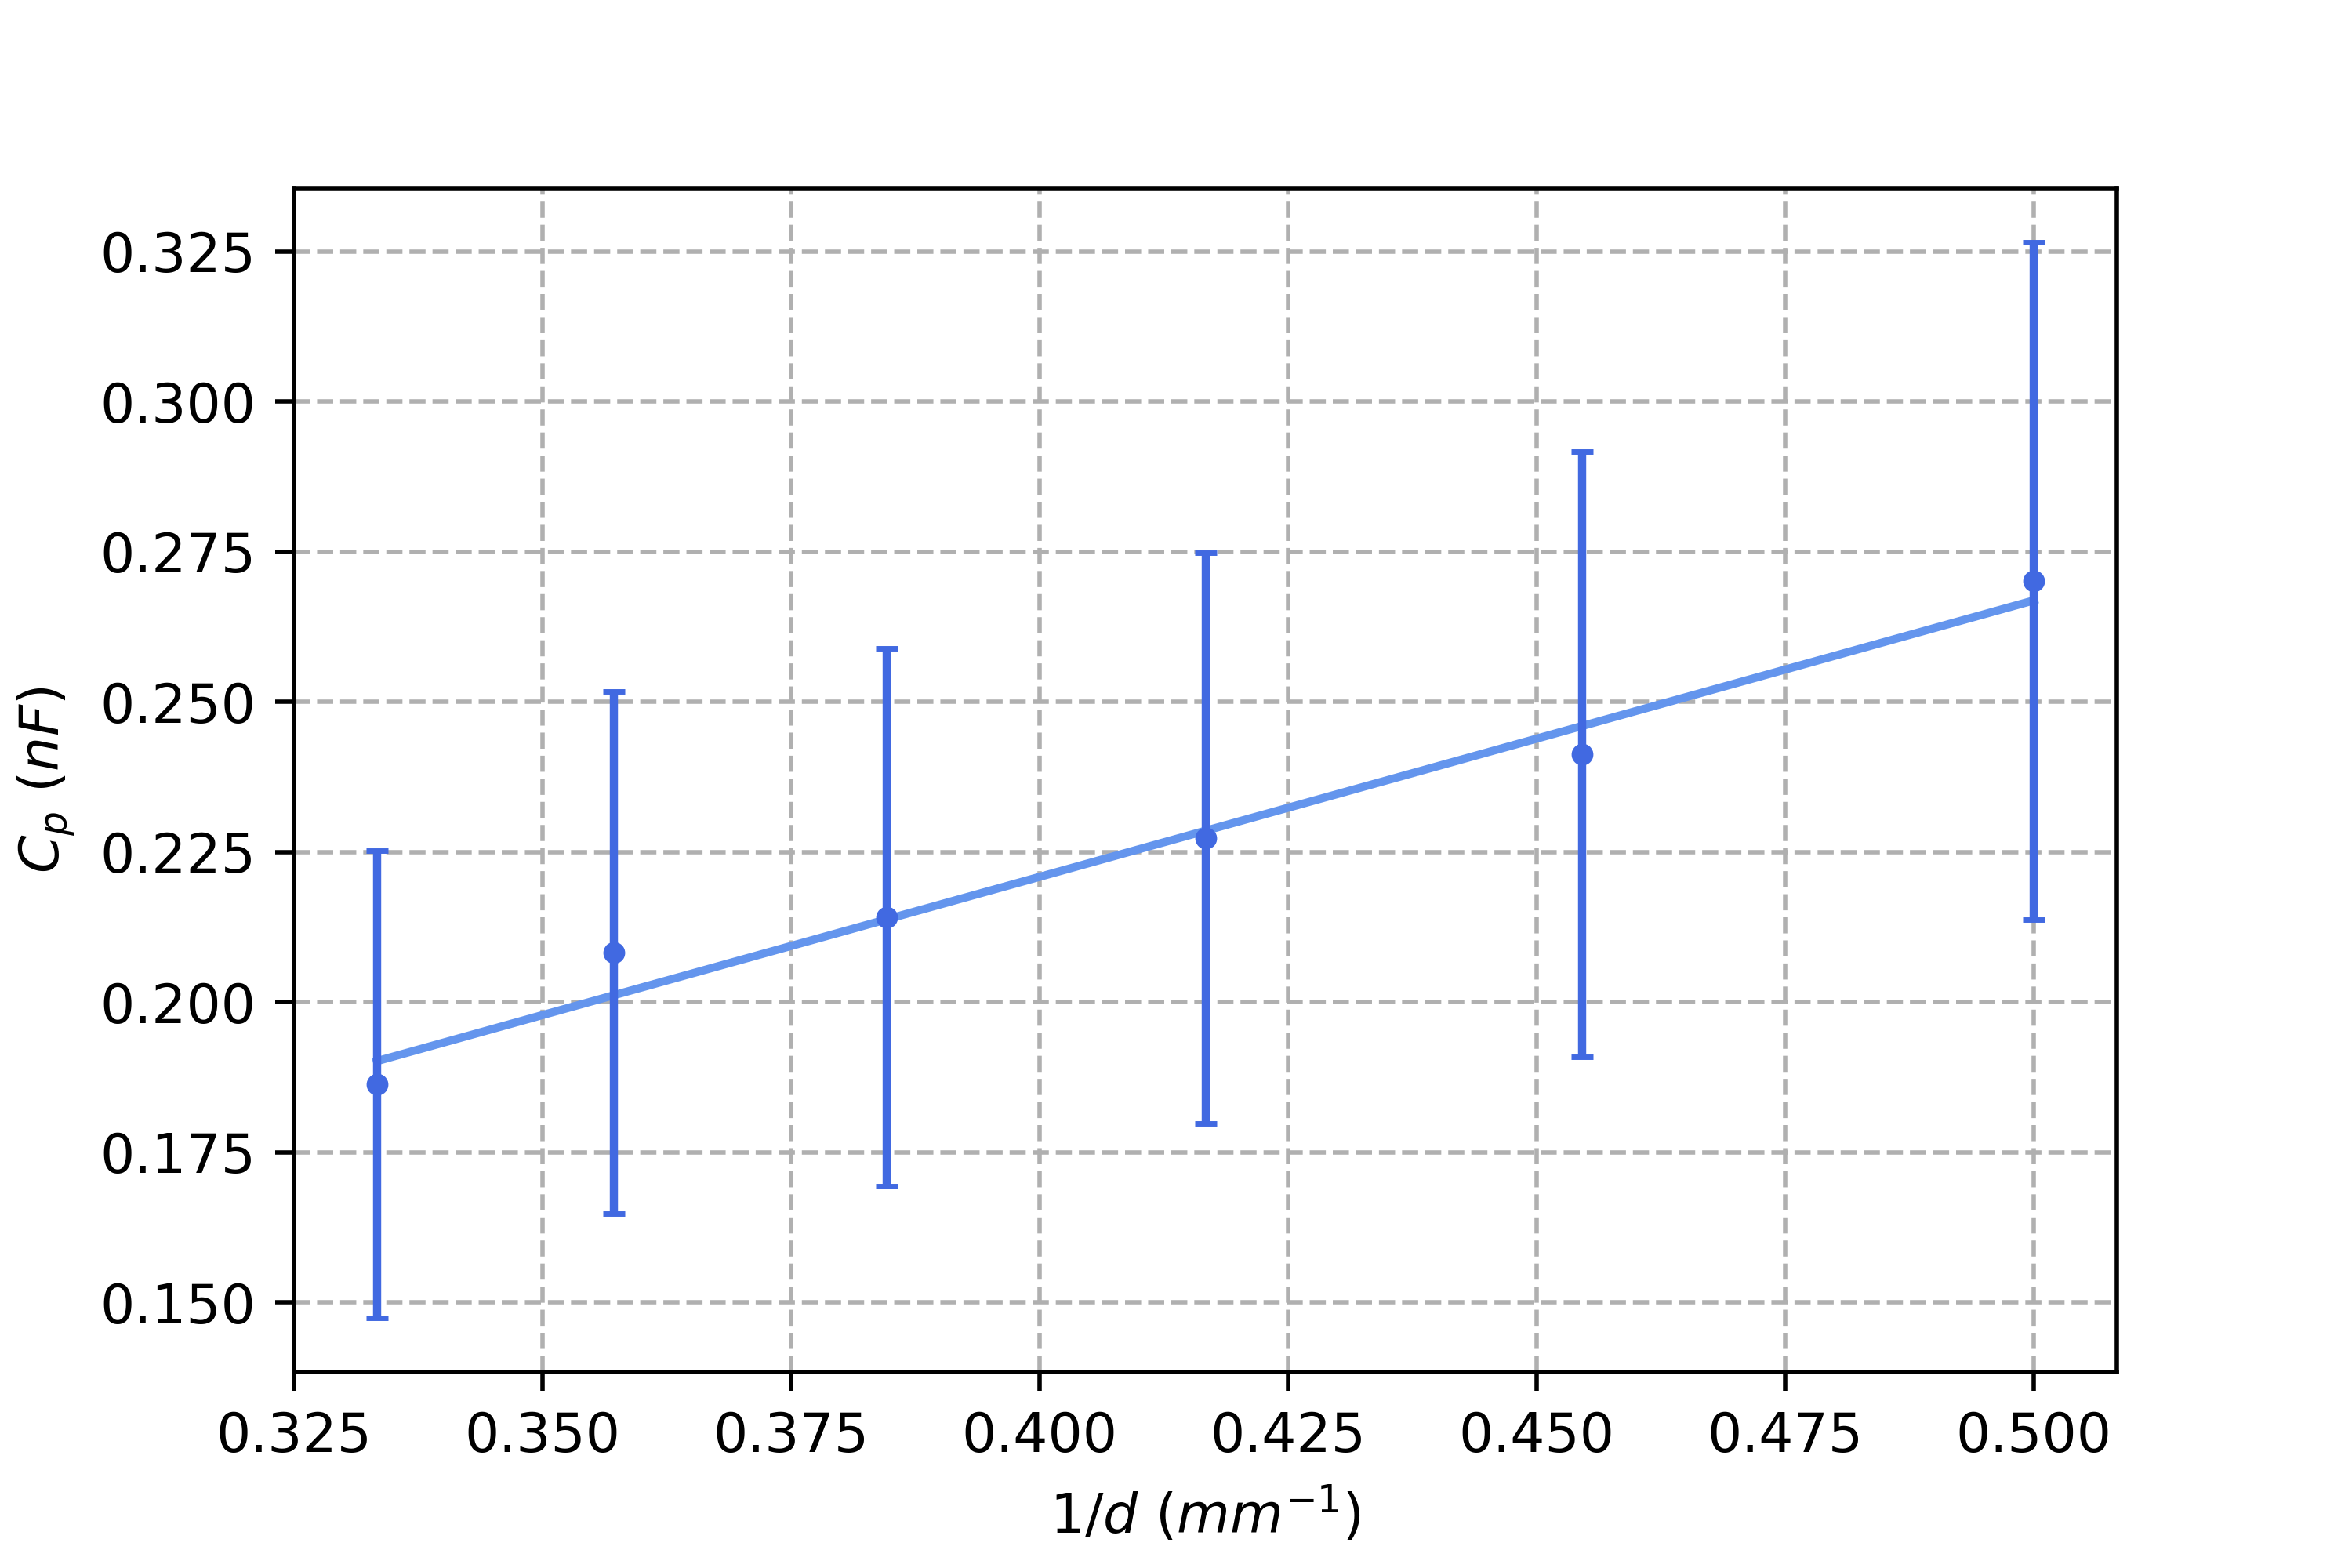
\includegraphics[scale=1]{plot1.png}
\caption{ajuste lineal de $C_p$ frente a $1/d$}
\label{Fig:regresion1}
\end{figure}
 
\newpage
 
\subsection{Parte 2:}

En este apartado tratamos de calcular la permitividad del vacío mediante una regresión lineal que enfrente la carga que adquiere el condensador frente al potencial entre las placas para una distancia entre ellas dada. Los datos obtenidos experimentalmente son:

$$ d = 2.5 \ (mm) \quad \quad s(d) = 0.1 \ (mm) $$

\begin{table}[h!] 	 \centering 
\begin{tabular}{|c|c|c|c|c|c|} 
\hline 
$V_0\ (kV)$ & $s(V_0) \ (kV)$ & $ V_M \ (V)$ & $s(V_M) \ (V)$ & $Q_0 \ (nC)  $ &  $s(Q_0) \ (nC)$ \\ \hline 
0.500  & 0.030 &  0.550 & 0.020 & 121 & 24 \\ 
1.000  & 0.060 &  1.125 & 0.021 & 247 & 49 \\ 
1.500  & 0.090 &  1.677 & 0.022 & 368 & 73 \\ 
2.000  & 0.120 &  2.130 & 0.023 & 468 & 93 \\ 
2.500  & 0.150 &  2.840 & 0.025 & 624 & 125 \\ 
3.000  & 0.180 &  3.670 & 0.027 & 807 & 161 \\ 
\hline
\end{tabular} 
\caption{datos de las medidas directas y las carga almacenada en $Q_0$} 
\label{tab:datos2} 
\end{table} 
 
 \newpage
 
Según las ecuaciones \ref{Ec:1} y \ref{Ec:3} tenemos que:

\begin{equation}
Q_0 = \frac{\varepsilon_0 S}{d} V_0 \longleftrightarrow Q_0 = a + b V_0
\end{equation}

y relacionando los parámetros con el ajuste lineal de $Q_0$ frente a $V_0$ podemos decir $a$ es un error dado por la calibración y la carga remanente, y b será:

\begin{equation}
b =  \frac{\varepsilon_0 S}{d} \Longrightarrow \varepsilon = \frac{b d}{S} = C_P
\end{equation}

Entonces podemos obtener los valores de la tabla \ref{tab:regresion2} de la regresión lineal (figura \ref{Fig:regresion2}):

\begin{table}[h!] 	 \centering 
\begin{tabular}{|c|c|c|c|c|} 
\hline 
$a \ (nC)$ & $s(a) \ (nC)$ & $ b \ (pF)$ & $s(b) \ (pF) $ & r  \\ \hline 
-6  & 35 &  252 & 35 & 0.997 \\ 
\hline
\end{tabular} 
\caption{valores de la regresión lineal (figura \ref{Fig:regresion2}).} 
\label{tab:regresion2} 
\end{table} 
 
Y de estos obtener el valor de la constante de permitividad del vacío: \\
 
\begin{equation}
\varepsilon_0 = 11.9 \cdot 10^{-12} \ (F/m) \quad \quad s(\varepsilon_0)=1.7 \cdot 10^{-12} \ (F/m)
\end{equation}
 
\begin{figure}[h!] \centering
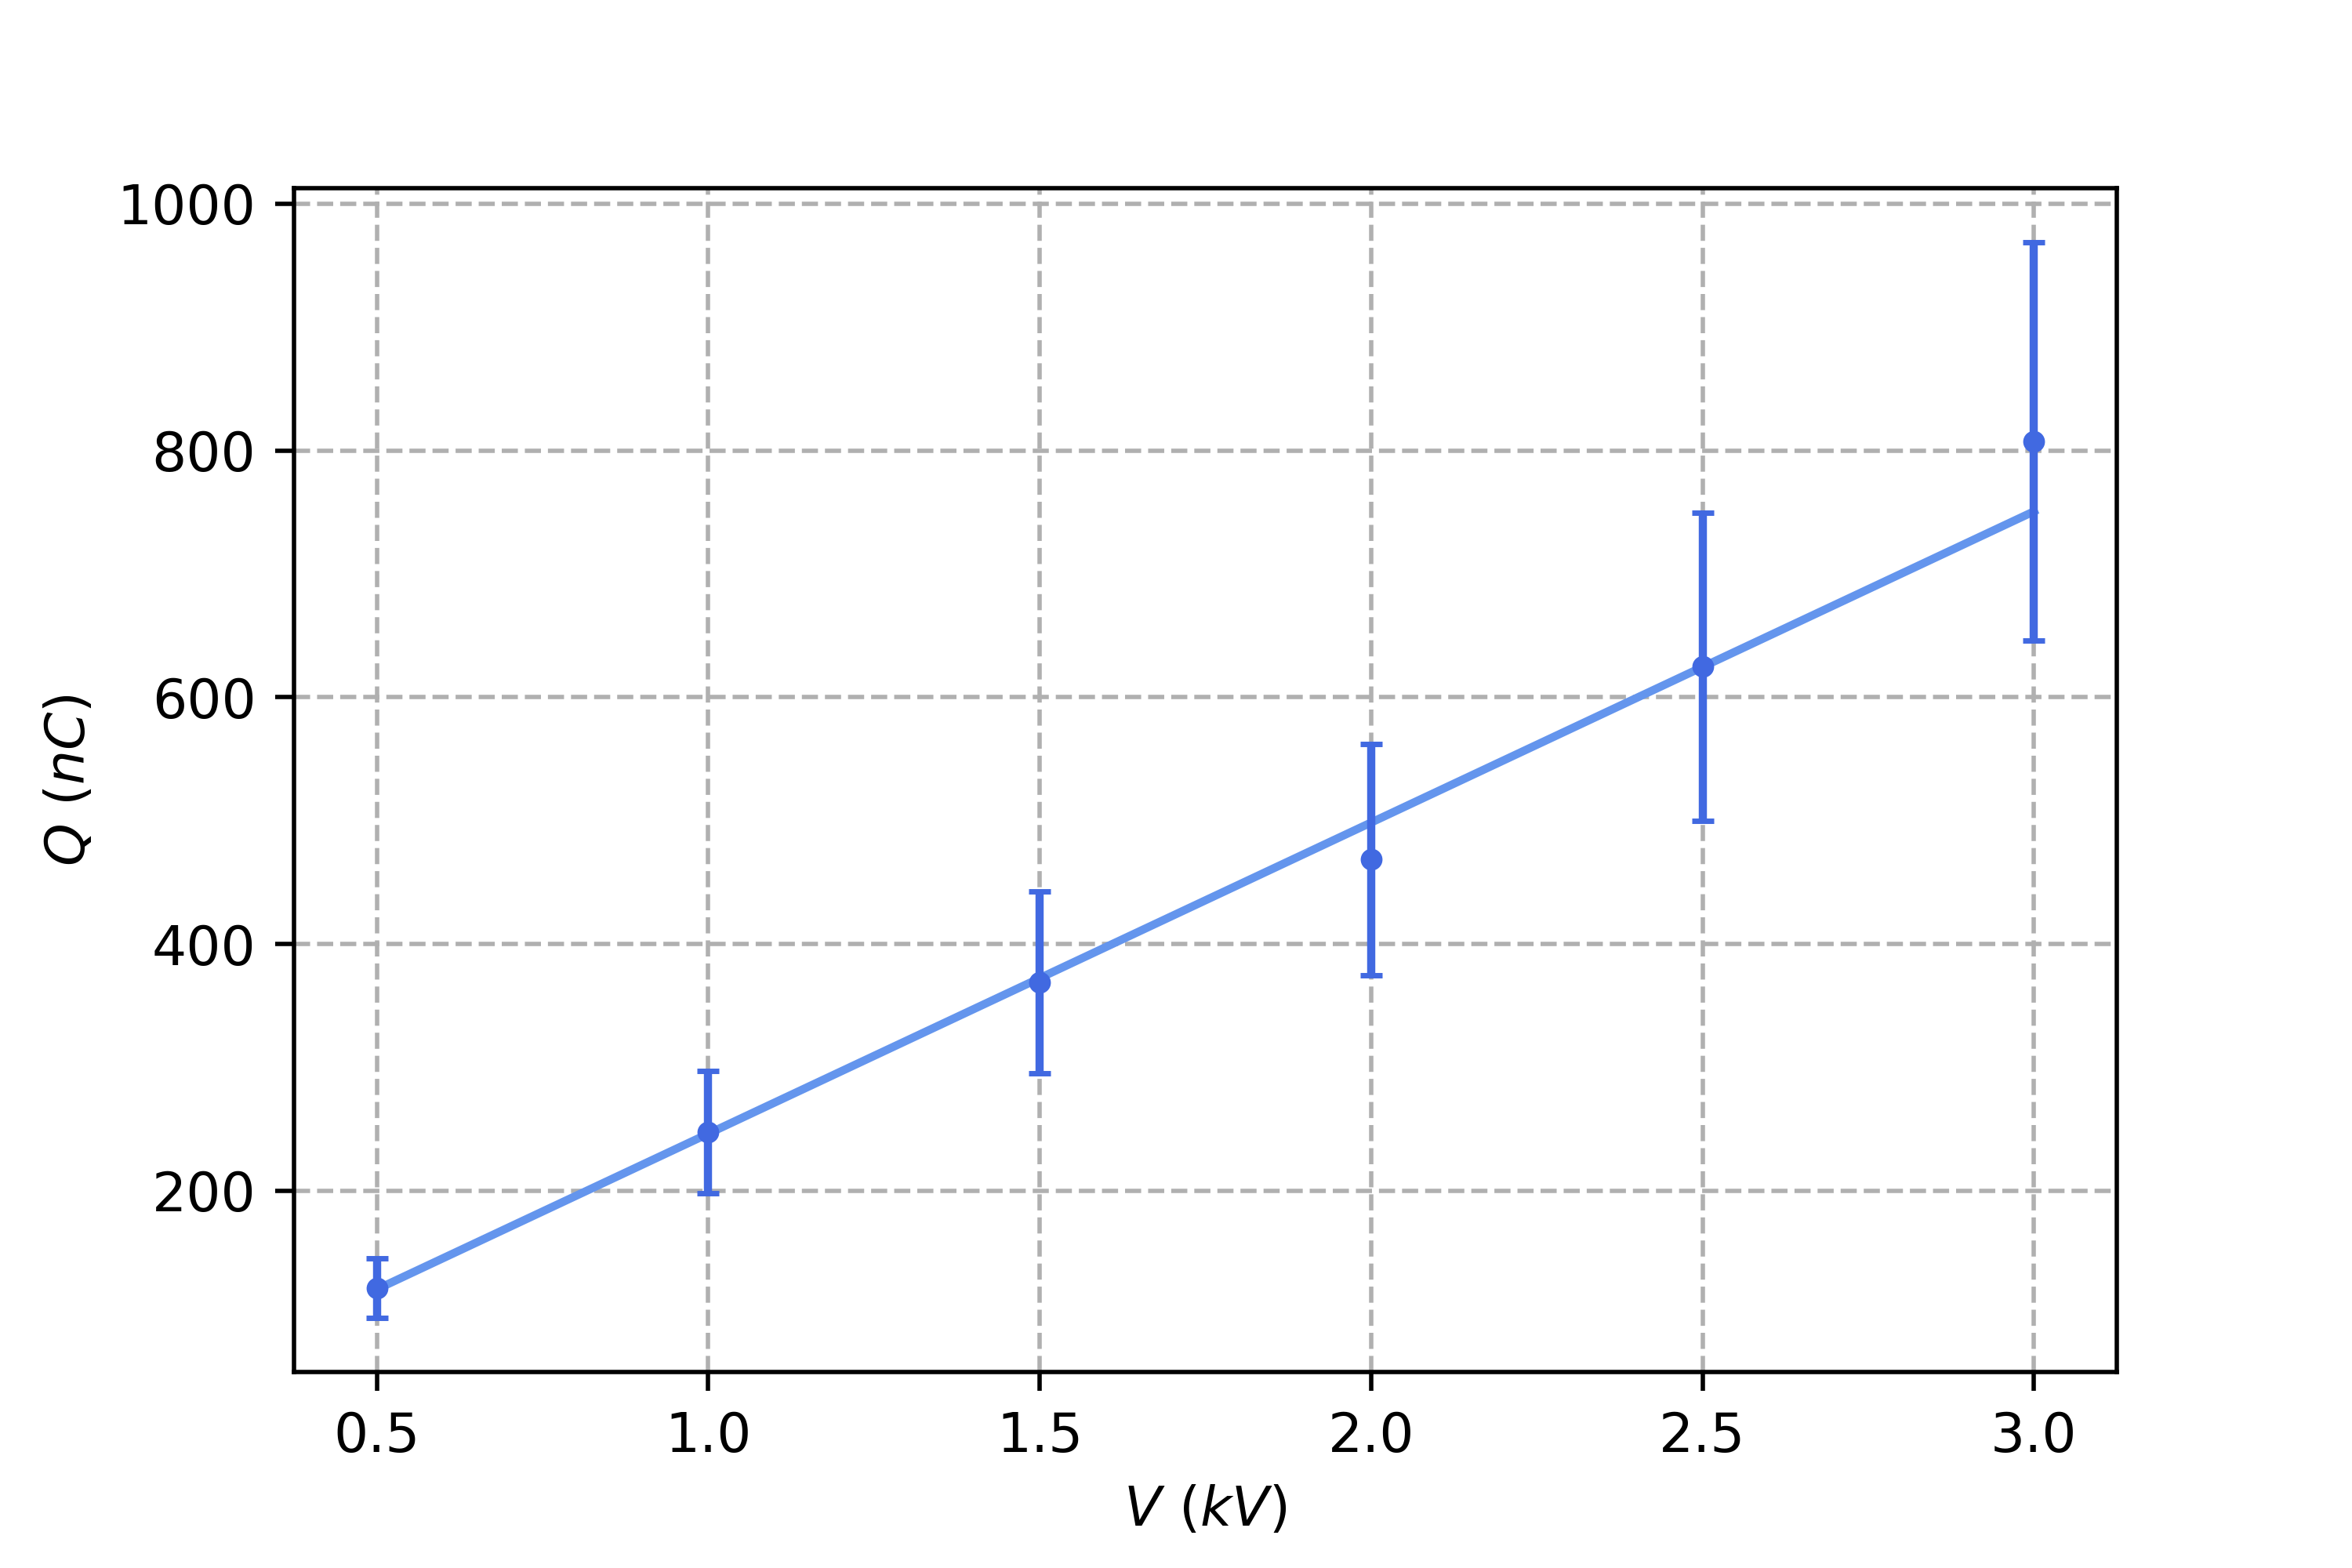
\includegraphics[scale=0.95]{plot2.png}
\caption{ajuste lineal de $Q_0$ frente a $V_0$}
\label{Fig:regresion2}
\end{figure}

\subsection{Parte 3}

En este apartado trataremos de calcular la permitividad relativa de un plástico realizando el cociente entre las capacidades de un condensador cuando hay medio dieléctrico y cuando no lo hay, usando la ecuación \ref{Ec:cociente}. Para calcular la capacidad haremos un ajuste lineal entre la carga almacenada y el voltaje dado entre las placas del condensador. Será importante la notación siguiente: $C_1$ se refiere a la capacidad con dieléctrico y $C_2$ sin dieléctrico. Obtenemos los siguientes datos:  \\

$$ d = 0.99 cm \quad \quad s(d) = 0.01 cm $$

\begin{table}[h!] 	 \centering 
\begin{tabular}{|c|c|c|c|c|c|} 
\hline 
$V_0\ (kV)$ & $s(V_0) \ (kV)$ & $ V_M \ (V)$ & $s(V_M) \ (V)$ & $Q_0 \ (nC)  $ &  $s(Q_0) \ (nC)$ \\ \hline 
1.000  & 0.060 &  0.980 & 0.021 & 215 & 43 \\ 
2.000  & 0.120 &  2.030 & 0.022 & 446 & 89 \\ 
3.000  & 0.180 &  3.150 & 0.025 & 693 & 138 \\ 
4.000  & 0.240 &  4.000 & 0.028 & 880 & 176 \\ 
5.000  & 0.300 &  5.040 & 0.032 & 1108 & 221 \\ 
\hline
\end{tabular} 
\caption{datos de las medidas directas y las carga almacenada en $Q_0$ con dieléctrico} 
\label{tab:datos3} 
\end{table} 
 
 \begin{table}[h!] 	 \centering 
\begin{tabular}{|c|c|c|c|c|c|} 
\hline 
$V_0\ (kV)$ & $s(V_0) \ (kV)$ & $ V_M \ (V)$ & $s(V_M) \ (V)$ & $Q_0 \ (nC)  $ &  $s(Q_0) \ (nC)$ \\ \hline 
1.000  & 0.060 &  0.370 & 0.020 & 81 & 16 \\ 
2.000  & 0.120 &  0.630 & 0.020 & 138 & 28 \\ 
3.000  & 0.180 &  1.020 & 0.021 & 224 & 45 \\ 
4.000  & 0.240 &  1.350 & 0.021 & 297 & 59 \\ 
5.000  & 0.300 &  1.600 & 0.022 & 352 & 70 \\ 
\hline
\end{tabular} 
\caption{datos de las medidas directas y las carga almacenada en $Q_0$ sin dieléctrico} 
\label{tab:datos4} 
\end{table} 
 
 
De la ecuación \ref{Ec:cociente} podemos deducir que la regresión lineal se puede asociar:

\begin{equation}
Q_0 = C_P V_0 \longleftrightarrow Q_0 = a + b V_0 
\end{equation}

donde claramente $a$ es el error por calibración y carga remanente y $b$ será

\begin{equation}
b = C_P
\end{equation}

pudiendo obtener los datos de (tab.\ref{tab:regresion3}) los ajustes lineales (\ref{Fig:regresion3}) de donde podemos obtener haciendo el cociente:


\begin{table}[h!] 	 \centering 
\begin{tabular}{|c|c|c|c|c|c|} 
\hline 
i & $a \ (nC)$ & $s(a) \ (nC)$ & $ C_i \ (pF)$ & $s(C_i) \ (pF) $ & r  \\ \hline 
1 & -9  & 67 &  226 & 36 & 0.9994 \\ \hline
2 & 10  & 24 &  69 & 12 & 0.996 \\ 
\hline
\end{tabular} 
\caption{pares de valores  para la regresión lineal \ref{Fig:regresion1}} 
\label{tab:regresion3} 
\end{table} 
 
\begin{equation}
\varepsilon_r = 3.28 \quad \quad s(\varepsilon_r) = 0.80
\end{equation}
 
\begin{figure}[h!] \centering
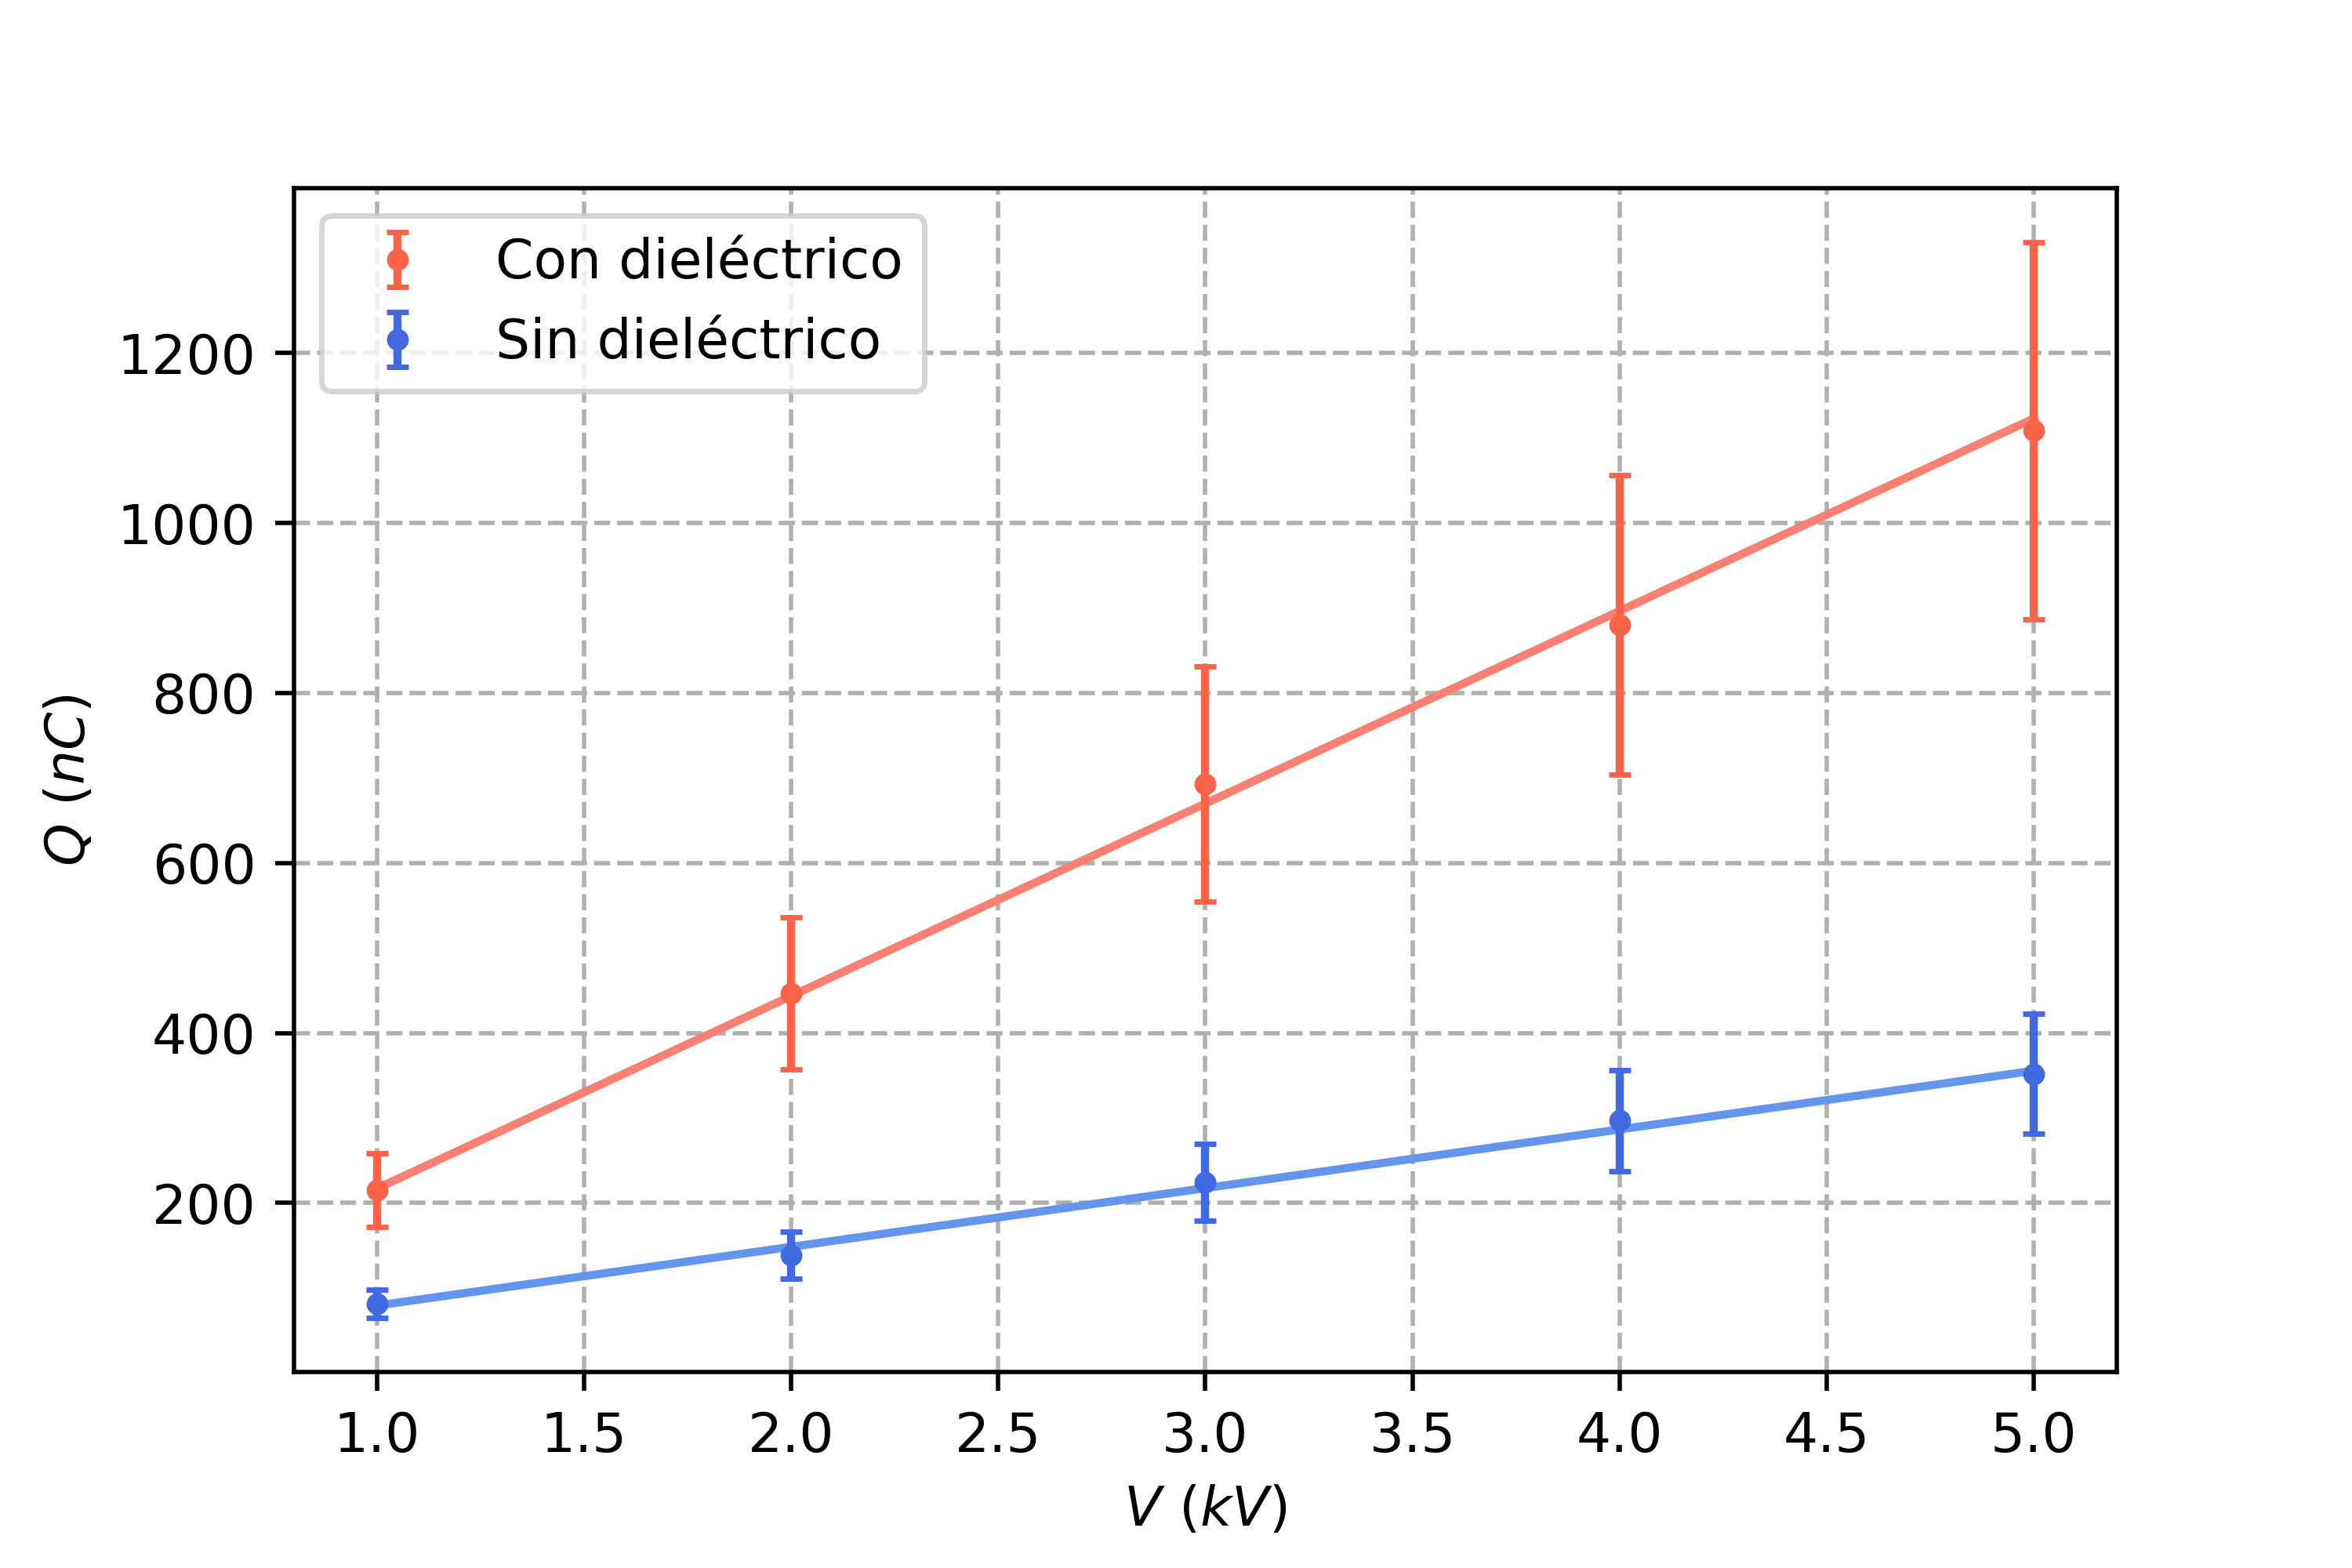
\includegraphics[scale=1]{plot3.png}
\caption{ajuste lineal de $Q_0$ frente a $V_0$ para el plástico y el vacío}
\label{Fig:regresion3}
\end{figure}
 
 
\section{Conclusiones}


Una vez hemos obtenido los resultados damos por finalizada la parte experimental de la práctica. En esta sección vamos a ir poco a poco extrayendo conclusiones de la práctica, respondiendo a algunas preguntas que surgen a lo largo de la práctica. En primer lugar vamos a tratar los resultados respondiendo a las siguientes preguntas: ¿Son concluyentes?¿Se puede mejorar la obtención de datos?¿Hay alguna otra fuente de incertidumbre que pasamos por alto?. Tras esto vamos a responder a otras preguntas que surgen de la experimentación. \\

Comencemos con las dos primeras partes de la práctica, que es obtener el valor de la permitividad del vacío. El valor teórico y los valores que nos dieron (siendo $\varepsilon_T$ el valor teórico, y $\varepsilon_1, \varepsilon_2$ los valores obtenidos en la parte 1 y 2 respectivamente) son :


\begin{equation} 
\begin{array}{llclllll}
\varepsilon_T   & = & 8.85 & \cdot 10^{-12} \ (F/m)  &  \ \ &   &   &   \\ 
\varepsilon_1 & = & 8.7 & \cdot 10^{-12} \ (F/m)  &  \ \ &  s(\varepsilon_1) & =  & 6.5 \cdot 10^{-12} \ (F/m)   \\ 
\varepsilon_2  & = & 11.9 & \cdot 10^{-12} \ (F/m) &  \ \ &  s(\varepsilon_2) & =  & 1.7  \cdot 10^{-12} \ (F/m)  \\ 
\end{array} 
\end{equation} 

Como podemos ver los dos que hemos calculado están en el mismo orden que el teórico, de hecho el primero de ellos se aproxima bastante, quedando dentro de su incertidumbre (aunque a decir verdad no es muy complicado, esta es relativamente hablando, elevada). Sin embargo la segunda, que a pesar de ser mas ``precisa'' se aleja mas de el valor real. Sin duda como aproximaciones son bastante buenas, e incluso podríamos realizar una media ponderada donde podríamos obtener un valor entorno a 10.5  pF/m. Ahora bien, porque realmente esta forma de calcular la constante dieléctrica no es todo lo exacta que se pudiera (solo se aproxima en el orden). Bien, sería un error achicar esto a la falta de precisión de los aparatos de medida, e incluso sería un error decir que mejorando la calidad de los instrumentos podrían obtenerse mejores valores. Esta claro que con mejores instrumentos los resultados serían mucho mas fiable, pero ese no es el punto de la pregunta. El quid de la cuestión es realmente la manera que tenemos de entender la capacidad de un condensador de cargas planas paralelas. \\

Si tuviéramos un condensador de placas plano paralelas infinitas la capacidad dada por la ecuación \ref{Ec:1} sería válida. Sin embargo, dicho valor, en problemas reales no es más que una aproximación, mas válida cuanto mayor sean las placas de nuestro condensador. En general dicha ecuación es una buena aproximación para grandes superficies, pero no es del todo correcta, aunque si que es lo suficientemente correcta  como para que los resultados estén a un $20 \%$ del valor real. \\

Además pueden influir otros factores, tales como la posible descarga de $Q_0$ al pasar la carga al otro condensador, factor que ya hemos mencionado y que se soluciona al hacer un cambio de configuración rápido; o por ejemplo que quede carga remanente en las placas del condensador de medida; inclusive puede ser que no hayamos dejado el suficiente tiempo de carga (ya hablaremos de esto mas adelante). Estos pequeños factores y otros muchos (humedad del aire, temperatura) son, al final, fuentes de incertidumbres que no se pueden controlar de manera directa, y  que la única manera de estudiarlas son haciendo muchas medidas, medidas que dado el tiempo que tenemos en el laboratorio no se pueden realizar. \\

Cabe mencionar que las coordenadas del origen de todas las regresiones tienen en su rango de incertidumbre el (0,0), por lo que está bien justificado la justificación de error de calibración y/o carga remanente. \\


%Una pregunta que nos podemos hacer al ver los resultados es que extrañamente con el proceso de la parte 1 obtenemos un dato mucho mas cercano al real que al realizar el proceso de la parte 2, es por qué sucede esto. Para hallar esto primero tenemos que ver las diferencias en las tomas de datos. Una de las diferencias mas notables es que cuando cambiar la distancia entre las placas es mucho mas lento que cambiar el voltaje. Esto puede parecer una trivialidad, pero cabe la posibilidad de que en esta diferencia de tiempo las cargas remanentes de ambos condensadores desaparezcan, y permitan una mejor medida posteriormente. También puede deberse a que al cambiar el voltaje en la fuente de alta tensión nos pasemos un poco de la cuenta tratando de dejar el voltaje requerido y eso permita la llegada de mas carga. Incluso puede que se deba algún fallo humano. \\

En la siguiente parte tratamos de calcular el valor de la permitividad relativa del plástico, enfrentándonos también a los mismos problemas que en los anteriores aparatados: los efectos de borde, perdidas por descarga, poco tiempo de carga... De todos modos el resultado que nos dio esta muy próximo al valor dado por Phywe: 2.9 pF/m. Comparándolos:

\begin{equation}
\mathrm{Teorico:} \ \ 2.9 \ pF/m \quad \quad \quad \quad \mathrm{Experimental:}  \ \ 3.3 \ pF/m
\end{equation}

quedando el valor teórico dentro del intervalo de incertidumbre del valor experimental. \\

En general los valores que nos dieron los resultados experimentales están bastante bien, no se pueden mejorar mucho, salvo por lo ya mencionado. Ahora vamos a responder a algunas cuestiones. \\

Uno de las razones por las que se puede hacer esta práctica es porque hemos supuesto que toda la carga del condensador $C_P$ se va al condensador de medida cuando ponemos la configuración 2. Esto se debe a dos factores, uno es que la carga del sistema es constante, y otro que el equilibrio del sistema ocurrirá cuando la diferencia de potencial entre las placas de ambos conductores sea la misma (esto es así porque este estado de equilibrio es el estado en el que la diferencia de potencial posible del sistema es mínima). En ese caso, como la capacidad de los condensadores es constante (sabemos que viene dado por factores geométricos), tenemos que para que los potenciales se igualen debe verificarse que:

\begin{equation}
\dfrac{C_P}{Q'_0}=\dfrac{C_M}{Q_M} \Longrightarrow \dfrac{Q_M}{Q'_{0}}=\dfrac{C_M}{C_P}
\end{equation} 

Entonces si $C_M \gg C_P$ tenemos que en el equilibrio $Q_M \gg Q'_0$, y como la carga es constante la carga inicial $Q_{0}$ debe ser:

\begin{equation}
Q_0 = Q_M + Q'_0 \approx Q_M
\end{equation}

Otra forma de verlo es que conectamos en realidad estamos conectando en paralelo ambos condensadores (figura \ref{Fig:configuracion2}), de tal manera que se tiene que verificar 

\begin{equation}
\varepsilon = \varepsilon_P + \varepsilon_M
\end{equation}
como $\varepsilon = 0 $ y por lo tanto $\varepsilon_P = \varepsilon_M$, (aparecería un signo derivado de tomar determinado sentido de recorrido, por lo que podemos escribir que se igualan). Entonces tenemos que:

$$ Q_0 / C_P = Q_M / C_M $$

y posteriormente un razonamiento igual que el anterior.


\section{Bibliografía} \label{Sec:7}

En esta sección simplemente mencionamos al guión de la práctica, que hemos usado sobretodo al escribir la introducción, material y montaje. Mención a que la imagen \ref{Fig:cofiguracion1} y \ref{Fig:configuracion2} se encontraban en este guion. Además hemos usado el manual de Phywe de la práctica \footnote{	\textcolor{blue}{\url{https://www.phywe.com/es/experimentos-sets/experimentos-universitarios/constante-dielectrica-de-diferentes-materiales_9228_10159/}}} donde podemos encontrar las incertidumbres de la mayoría de la prácticas, menos la del polímetro, que sacamos dichos valores de la hoja de especificaciones que nos dio la inteligencia artificial GPT3. 


%Otra de las cuestiones que están implicadas en esta práctica es la del tiempo de respuesta. En esta parte vamos a calcular el tiempo de respuesta de nuestro sistema (para cargar las placas del condensador) y ver si hemos considerado un tiempo de carga adecuado o no. El tiempo de relajación $\tau$ de nuestro circuito en la configuración 1 vendrá dado por:

%\begin{equation}
%\tau =  R \cdot C = 10 \cdot 10^6 \cdot \dfrac{\varepsilon S}{d}
%\end{equation}

%Por ejemplo para el caso de la parte 2 tenemos que (y usando el valor teórico de $\varepsilon_0$) tenemos que tardaría 0.019 segundo, y en el caso de la parte 3 con plástico tardaría 0.15 segundos, lo cual hemos visto que no es cierto. 
 
\end{document}
